\chapter{Specifikacija programske potpore}
		
	\section{Funkcionalni zahtjevi}
			\noindent \textbf{Dionici:}
			
			\begin{packed_enum}
				
				\item Roditelj
				\item Zdravstveni djelatnik	
				\begin{packed_enum}
					\item Liječnik
					\item Pedijatar
				\end{packed_enum}			
				\item Administrator
				\item Vanjski sudionik
				\begin{packed_enum}
					\item Poslodavac
					\item Škola/vrtić
				\end{packed_enum}
				\item Razvojni tim
			\end{packed_enum}
			
			\noindent \textbf{Aktori i njihovi funkcionalni zahtjevi:}
			
			
			\begin{packed_enum}
				\item  \underbar{Neregistrirani/neprijavljeni korisnik (inicijator) može:}
				
				\begin{packed_enum}
					\item se registrirati u sustav, stvoriti novi korisnički račun za koji su mu potrebni ime, prezime,  lozinka, e-mail adresa, spol, datum rođenja, adresa i OIB
				\item se prijaviti u sustav pomoću korisničkog računa i lozinke
				\end{packed_enum}
			
				\item  \underbar{Roditelj (inicijator) može:}
				\begin{packed_enum}
					\item vidjeti svoj profil i profile svoje djece
					\item pregledavati naslovnu stranicu s prikazom zakazanih termina i obavijestima od strane liječnika ili pedijatra
					\item prijaviti željeni termin pregleda ili poslati nalaze privatnih pregleda liječniku ili pedijatru
					\item pregledavati prijašnji popis bolesti i pregleda svoje djece
					\item odjaviti se iz aplikacije
				\end{packed_enum}
			
				\item  \underbar{Zdravstveni djelatnik (liječnik/pedijatar) (inicijator) može:}
				\begin{packed_enum}
					\item potvrditi ili odbiti zahtjev za pregledom dijeteta od strane roditelja
					\item vidjeti profil pacijenata te povijest pregleda i nalaza
					\item evidentirati preglede djece i događaje na istim
					\item poslati povratnu informaciju vezano uz nalaz roditelju
					\item pohraniti novi nalaz s povratnom informacijom
					\item izdati i odobriti ispričnicu u slučaju bolesti dijeteta
					\item preporučiti preporuku o bolovanju za roditelja bolesnog djeteta u slučaju pedijatra, a izdati i odobriti preporuku o bolovanju za roditelja bolesnog djeteta u slučaju liječnika
					\item odjaviti se iz aplikacije
				\end{packed_enum}
				
				\item  \underbar{Administrator (inicijator) može:}
				\begin{packed_enum}
					\item vidjeti popis svih korisnika i njihovih profila te profile njihove djece
					\item brisati i mijenjati razinu ovlasti korisnika aplikacije (roditelj, pedijatar/liječnik, administrator)
					\item dodati ili obrisati korisnika
					\item izmjeniti profile korisnika
					\item povezivati liječnike/pedijatre s roditeljima
					\item odjaviti se iz aplikacije
				\end{packed_enum}
				
				\item  \underbar{Vanjski sudionik (poslodavac/škola/vrtić) (sudionik) može:}
				\begin{packed_enum}
					\item zaprimiti ispričnicu/molbu za bolovanjem od strane liječnika/pedijatra
				\end{packed_enum}
			
				\item  \underbar{Baza podataka (sudionik) može:}
				\begin{packed_enum}
				\item pohranjuje sve podatke o korisnicima i njihovim ovlastima
				\item pohranjuje sve podatke o pregledima i bolestima pacijenata
				\item pohranjuje veze između liječnika/pedijatra i pacijenata
				\item pohranjuje zakazane termine i termine na čekanju za odobrenje
				\item pohranjuje ispričnice, preporuke o bolovanju i nalaze pacijenata
				\end{packed_enum}
			\end{packed_enum}
			
			\eject 
			
			
				
			\subsection{Obrasci uporabe}
				
				\subsubsection{Opis obrazaca uporabe}
				
					\noindent \underbar{\textbf{UC1 - Registriraj se}}
					\begin{packed_item}
	
						\item \textbf{Glavni sudionik: } Neregistrirani korisnik
						\item  \textbf{Cilj:} Kreirati korisnički račun za pristup sustavu
						\item  \textbf{Sudionici:} Baza podataka
						\item  \textbf{Preduvjet:} -
						\item  \textbf{Opis osnovnog tijeka:}
						
						\item[] \begin{packed_enum}
	
							\item Korisnik odabire opciju "Nemate račun? Registrirajte se!"
							\item Sustav vodi korisnika na putanju "/registracija" 
							\item Korisnik unosi potrebne podatke (ime, prezime, OIB, email, lozinku, potvrdu lozinke, spol, datum rođenja, adresu)
							\item Korisnik potvrđuje unos podataka odabirom akcije "Registriraj se"
							\item Sustav provjerava (ime, prezime, OIB, email, lozinku, potvrdu lozinke, spol, datum rođenja, adresu) i utvrđuje da je unos uspješan te vodi korisnika na naslovnu stranicu s putanjom "/naslovna"
						\end{packed_enum}
						
						\item  \textbf{Opis mogućih odstupanja:}
						
						\item[] \begin{packed_item}
							
							\item[5.a] Sustav radi provjere i utvrđuje da unos podataka nije uspješan te obavještava korisnika porukom. Sustav nastavlja izvođenje scenarija u koraku 3. 
	
							\item[5.b] Korisnik odabire opciju "Već imate račun? Prijavite se!" te ga sustav vodi na sučelje za prijavu na putanji "/prijava"
						
						\end{packed_item}
								
					\end{packed_item}
					
					
						\noindent \underbar{\textbf{UC2 - Prijavi se}}
					\begin{packed_item}
						
						\item \textbf{Glavni sudionik: }Korisnik
						\item  \textbf{Cilj:} Prijava u sustav s postojećim računom
						\item  \textbf{Sudionici:} Baza podataka
						\item  \textbf{Preduvjet:} Korisnik ima registrirani račun i nalazi se na putanji "/prijava"
						\item  \textbf{Opis osnovnog tijeka:}
						
						\item[] \begin{packed_enum}
							\item Korisnik unosi potrebne podatke (email, lozinku)
							\item Korisnik potvrđuje unos podataka odabirom akcije "Prijavi se"
							\item Sustav provjerava (email, lozinku) i utvrđuje da je unos uspješan te vodi korisnika na naslovnu stranicu s putanjom "/naslovna"
						\end{packed_enum}
						
						\item  \textbf{Opis mogućih odstupanja:}
						
						\item[] \begin{packed_item}
							
							\item[3.a] Sustav radi provjere i utvrđuje da prijava nije uspješan te obavještava korisnika porukom. Sustav nastavlja izvođenje scenarija u koraku 1. 
							
							\item[3.b] Korisnik odabire opciju "Nemate račun? Registrirajte se!" te ga sustav vodi na sučelje za registraciju na putanji "/registracija"							
						\end{packed_item}
						
					\end{packed_item}
					
					
				\noindent \underbar{\textbf{UC3 - Pregledaj naslovnu stranicu}}
				\begin{packed_item}
					
					\item \textbf{Glavni sudionik: }Roditelj, Administrator, Liječnik ili Pedijatar
					\item  \textbf{Cilj:} Pregled novih obavijesti i zakazanih termina od zadnje prijave
					\item  \textbf{Sudionici:} Baza podataka
					\item  \textbf{Preduvjet:} Korisnik sustava je prijavljen
					\item  \textbf{Opis osnovnog tijeka:}
					
					\item[] \begin{packed_enum}
						
						\item Korisnik odabire karticu "Naslovna" kod bočnog izbornika
						\item Sustav vodi korisnika na naslovnu stranicu s putanjom "/naslovna" i radi dohvaćanje potrebnih podataka (datum, vrijeme te ime, prezime, OIB medicinskog osoblja i dijeteta)
						\item Sustav prikazuje zakazene termine grupirane u sučelju "Zakazani termini", a nove obavijesti u sučelju "Nove obavijesti"
					\end{packed_enum}
					
						\item  \textbf{Opis mogućih odstupanja:}
					
					\item[] \begin{packed_item}
						
						\item[3.a] Sustav prilikom dohvaćanja podataka nailazi na grešku te obavještava korisnika porukom
						
						\item[3.b] Sustav prilikom dohvaćanja podataka utvrđuje da nema novih obavijesti ili zakazanih termina te obavještava korisnika porukom				
					\end{packed_item}
					
				\end{packed_item}
				
				
				\noindent \underbar{\textbf{UC4 - Pregledaj korisnički profil}}
				\begin{packed_item}
					
					\item \textbf{Glavni sudionik: }Roditelj, Administrator, Liječnik ili Pedijatar
					\item  \textbf{Cilj:} Pregled osobnih podataka korisnika i njegove dijece
					\item  \textbf{Sudionici:} Baza podataka
					\item  \textbf{Preduvjet:} Korisnik sustava je prijavljen
					\item  \textbf{Opis osnovnog tijeka:}
					
					\item[] \begin{packed_enum}
						\item Korisnik odabire karticu "Profil" kod bočnog izbornika
						\item Sustav vodi korisnika na stranicu s putanjom "/naslovna/profil"
						\item Sustav radi dohvaćanje podataka o korisniku (ime, prezime, OIB, spol, adresa, datum rođenja, email) i djeci (ime, prezime, OIB, spol, adresa, datum rođenja)
						\item Sustav prikazuje korisničke podatke grupirane u sučelju "MOJ PROFIL", a podatke o djeci grupirane u sučelju "PROFILI DJECE"
					\end{packed_enum}
					
					\item  \textbf{Opis mogućih odstupanja:}
					
					\item[] \begin{packed_item}
						
						\item[3.a] Korisnik sustava ima ulogu Administrator, Liječnik ili Pedijatar te sustav ne dohvaća podatke o dijeci
						\item[4.a] Korisnik sustava ima ulogu Roditelj i sustav ne prikazuje sučelje "PROFILI DJECE" nego obaviještava korisnika porukom da nema dijece
						\item[4.b] Korisnik sustava ima ulogu Administrator, Liječnik ili Pedijatar te sustav ne prikazuje sučelje "PROFILI DJECE"
					\end{packed_item}
					
				\end{packed_item}
				
				
				\noindent \underbar{\textbf{UC5 - Pregledaj popis povijesti pregleda i nalaza}}
				\begin{packed_item}
					
					\item \textbf{Glavni sudionik: }Roditelj, Liječnik ili Pedijatar
					\item  \textbf{Cilj:} Pregled popisa povijesti pregleda i nalaza djece/pacijenata
					\item  \textbf{Sudionici:} Baza podataka
					\item  \textbf{Preduvjet:} Korisnici sustava je prijavljen
					\item  \textbf{Opis osnovnog tijeka:}
					
					\item[] \begin{packed_enum}
						\item Korisnik s ulogom Roditelj odabire karticu "Popis pregleda" dok korisnik s ulogom Liječnik ili Pedijatar odabire karticu "Kartoni pacijenata" kod bočnog izbornika
						\item Sustav vodi korisnika na stranicu s putanjom "/naslovna/popisPregleda"
						\item Korisnik odabire željeno dijete iz padajućeg izbornika
						\item Na temelju odabira sustav radi dohvaćanje osnovnih podataka o prijašnjim pregledima (datum, vrijeme, ime, prezime, OIB i uloga medicinskog osoblja) i nalazima (datum, vrijeme, postojanje povratne informacije)
						\item Sustav u obliku liste prikazuje osnovne podatke o pregledima grupirane u sučelju "POVIJEST PREGLEDA", a osnovne podatke o nalazima u sučelju "POVIJEST NALAZA"
						\item Odabirom akcije "Otvori" sustav vodi korisnika na putanju "/naslovna/pregled/id" ili "/naslovna/nalaz/id"
					\end{packed_enum}
					
						\item  \textbf{Opis mogućih odstupanja:}
					
					\item[] \begin{packed_item}
						
						\item[4.a] Sustav prilikom dohvaćanja podataka nailazi na grešku te obavještava korisnika porukom
						
						\item[4.b] Sustav prilikom dohvaćanja podataka utvrđuje da dijete/pacijent nema prijašnjih pregleda ili nalaza te obavještava korisnika porukom					
					\end{packed_item}
					
				\end{packed_item}
				
				
				
				\noindent \underbar{\textbf{UC6 - Pregledaj odabrani pregled}}
				\begin{packed_item}
					
					\item \textbf{Glavni sudionik: }Roditelj, Liječnik ili Pedijatar
					\item  \textbf{Cilj:} Pregled svih informacija vezanih uz odabrani pregled
					\item  \textbf{Sudionici:} Baza podataka
					\item  \textbf{Preduvjet:} Sustav je obavio scenarij UC5
					\item  \textbf{Opis osnovnog tijeka:}
					
					\item[] \begin{packed_enum}
						\item Na temelju identifikatora "id" trenutne putanje "/naslovna/pregled/id" sustav radi dohvaćanje svih podataka o pregledu (datum, vrijeme, ime, prezime, OIB i uloga medicinskog osoblja, opis i trajanje simptoma, opis fizičkog pregleda, opis dijagnoze, propisani lijekovi, preporučeno daljnje liječenje, podaci o izdanoj ispričnici i preporuci o bolovanju) i dijetetu/pacijentu (ime, prezime, OIB, spol, adresa, datum rođenja)
						\item Sustav prikazuje dohvaćene podatke
						\item Korisnik akcijom "Preuzmi" preuzima ispričnicu i/ili preporuku za bolovanjem
					\end{packed_enum}
					
					\item  \textbf{Opis mogućih odstupanja:}
					
					\item[] \begin{packed_item}
						
						\item[1.a] Sustav prilikom dohvaćanja podataka nailazi na grešku te obavještava korisnika porukom
						
						\item[3.a] Sustav utvrđuje da nije izdana ispričnica i/ili preporuka o bolovanju i ne dozvoljava akciju "Preuzmi"			
					\end{packed_item}
					
				\end{packed_item}
				
				
				\noindent \underbar{\textbf{UC7 - Pregledaj odabrani nalaz}}
				\begin{packed_item}
					
					\item \textbf{Glavni sudionik: }Roditelj, Liječnik ili Pedijatar
					\item  \textbf{Cilj:} Pregled svih informacija vezanih uz odabrani nalaz
					\item  \textbf{Sudionici:} Baza podataka
					\item  \textbf{Preduvjet:} Sustav je obavio scenarij UC5
					\item  \textbf{Opis osnovnog tijeka:}
					
					\item[] \begin{packed_enum}
						\item Na temelju identifikatora "id" trenutne putanje "/naslovna/nalaz/id" sustav radi dohvaćanje svih podataka o nalazu (datum, vrijeme, nalaz, dodatna povratna informacija) i dijetetu/pacijentu (ime, prezime, OIB, spol, adresa, datum rođenja)
						\item Sustav prikazuje dohvaćene podatke
						\item Korisnik akcijom "Preuzmi" preuzima nalaz kao datoteku
					\end{packed_enum}
					
					\item  \textbf{Opis mogućih odstupanja:}
					
					\item[] \begin{packed_item}
						
						\item[1.a] Sustav prilikom dohvaćanja podataka nailazi na grešku te obavještava korisnika porukom	
					\end{packed_item}
					
				\end{packed_item}		
				
				
				
				
				\noindent \underbar{\textbf{UC8 - Pošalji novi zahtjev za termin pregleda}}
				\begin{packed_item}
					\item \textbf{Glavni sudionik: }Roditelj
					\item  \textbf{Cilj:} Poslati novi zahtjev za termin pregleda djeteta
					\item  \textbf{Sudionici:} Baza podataka, Liječnik, Pedijatar
					\item  \textbf{Preduvjet:} Roditelj je prijavljen u sustav i dijetetu je dodijeljeni liječnik ili pedijatar
					\item  \textbf{Opis osnovnog tijeka:}
					\item[] \begin{packed_enum}
						\item Roditelj odabire karticu "Novi Termin" kod bočnog izbornika
						\item Sustav vodi korisnika na stranicu s putanjom "/naslovna/noviTermin" i prikazuje formu za unos podataka o terminu pregleda
						\item Korisnik odabire željeno dijete i medicinsko osoblje iz padajućih izbornika
						\item Korisnik označava opciju "Želim zakazati termin"
						\item Sustav prikazuje dodatna polja za unos datuma i vremena
						\item Korisnik ispunjava polja i odabirom akcije "Pošalji" šalje podatke
						\item Sustav obrađuje podatke i porukom obavještava korisnika o uspješnom slanju
						
						\item[] \begin{packed_item}
						\item[3.a] Sustav prilikom dohvaćanja podataka nailazi na grešku te ne dozvoljava slanje novog termina pregleda
						
						\item[3.b] Sustav utvrđuje da dijete nema dodijeljenog liječnika i/ili pedijatra i ne dozvoljava slanje novog termina pregleda
						
						\item[7.a] Sustav prilikom obrade podataka obavještava korisnika da nisu popunjena sva obavezna polja porukom
						
						\item[7.b] Sustav prilikom slanja podataka nailazi na grešku te obavještava korisnika porukom o neuspješnom slanju	
					\end{packed_item}
				\end{packed_enum}
						
					\end{packed_item}
					
					
					
					\noindent \underbar{\textbf{UC9 - Pošalji novi nalaz dijeteta}}
					\begin{packed_item}
						
						\item \textbf{Glavni sudionik: }Roditelj
						\item  \textbf{Cilj:} Poslati i pohraniti novi nalaz
						\item  \textbf{Sudionici:} Baza podataka, Liječnik, Pedijatar
						\item  \textbf{Preduvjet:} Roditelj je prijavljen i ima dodijeljenu dijecu
						\item  \textbf{Opis osnovnog tijeka:}
						
						\item[] \begin{packed_enum}
							\item Roditelj odabire karticu "Novi Termin" kod bočnog izbornika
							\item Sustav vodi Roditelja na stranicu s putanjom "/naslovna/noviTermin" te prikazuje formu za prijenos nalaza
							\item Roditelj odabire željeno dijete i medicinsko osoblje iz padajućih izbornika
							\item Roditelj odabire opciju "Želim prenijeti nalaz"
							\item Sustav prikazuje dodatna polja za prijenos nalaza
							\item Roditelj prenosi nalaz akcijom "Odaberi datoteku"
							\item Roditelj traži povratnu informaciju odabirom opcije "Želim povratnu informaciju"
							\item Roditelj odabire akciju "Pošalji" za slanje nalaza
							\item Sustav obrađuje podatke i porukom obavještava korisnika o uspješnom slanju
						\end{packed_enum}
						
						\item  \textbf{Opis mogućih odstupanja:}
						
						\item[] \begin{packed_item}
							\item[3.a] Sustav prilikom dohvaćanja podataka nailazi na grešku te ne dozvoljava slanje novog nalaza
							
							\item[3.b] Sustav utvrđuje da dijete nema dodijeljenog liječnika i/ili pedijatra i ne dozvoljava slanje novog nalaza	
							
							\item[9.a] Sustav prilikom obrade podataka obavještava korisnika da nisu popunjena sva obavezna polja porukom
							
							\item[9.b] Sustav prilikom slanja podataka nailazi na grešku te obavještava korisnika porukom o neuspješnom slanju
						\end{packed_item}
					\end{packed_item}
					
					
					
					
					
					\noindent \underbar{\textbf{UC10 - Pošalji novi nalaz pacijenta}}
					\begin{packed_item}
						
						\item \textbf{Glavni sudionik: }Liječnik ili Pedijatar
						\item  \textbf{Cilj:} Poslati i pohraniti novi nalaz
						\item  \textbf{Sudionici:} Baza podataka, Roditelj
						\item  \textbf{Preduvjet:} Liječnik/Pedijatar je prijavljen i ima dodijeljene pacijente
						\item  \textbf{Opis osnovnog tijeka:}
						
						\item[] \begin{packed_enum}
							\item Liječnik/Pedijatar odabire karticu "Novi Nalaza" kod bočnog izbornika
							\item Sustav vodi Liječnika/Pedijatra na stranicu s putanjom "/naslovna/noviNalaz" te prikazuje formu za prijenos nalaza
							\item Liječnik/Pedijatar odabire željenog pacijenta iz padajućih izbornika
							\item Sustav prikazuje dodatna polja za prijenos nalaza
							\item Liječnik/Pedijatar prenosi nalaz akcijom "Odaberi datoteku"
							\item Liječnik/Pedijatar unosi povratnu informaciju u tekstualno polje
							\item Liječnik/Pedijatar odabire akciju "Pošalji" za slanje nalaza
							\item Sustav obrađuje podatke i porukom obavještava korisnika o uspješnom slanju
						\end{packed_enum}
						
						\item  \textbf{Opis mogućih odstupanja:}
						
						\item[] \begin{packed_item}
							\item[3.a] Sustav prilikom dohvaćanja podataka nailazi na grešku te ne dozvoljava slanje novog nalaza
							
							\item[3.b] Sustav utvrđuje da Liječnik/Pedijatar nema dodijeljenih pacijenata i ne dozvoljava slanje novog nalaza
							
							\item[8.a] Sustav prilikom obrade podataka obavještava korisnika da nisu popunjena sva obavezna polja porukom
							
							\item[8.b] Sustav prilikom slanja podataka nailazi na grešku te obavještava korisnika porukom o neuspješnom slanju
						\end{packed_item}
					\end{packed_item}
					
					
					
					
					\noindent \underbar{\textbf{UC11 - Otkaži zakazani termin}}
				\begin{packed_item}
					
					\item \textbf{Glavni sudionik: }Roditelj, Liječnik ili Pedijatar
					\item  \textbf{Cilj:} Otkazati zakazani termin
					\item  \textbf{Sudionici:} Baza podataka, Liječnik, Pedijatar, Roditelj
					\item  \textbf{Preduvjet:} Korisnik je prijavljen
					\item  \textbf{Opis osnovnog tijeka:}
					
					\item[] \begin{packed_enum}
						\item Roditelj odabire karticu "Novi Termin" dok Liječnik/Pedijatar odabire karticu "Termini na čekanju" kod bočnog izbornika
						\item Sustav vodi Roditelja na stranicu s putanjom "/naslovna/noviTermin" dok Liječnika/Pedijatra vodi na stranicu s putanjom "/naslovna/terminiNaCekanju"
						\item Sustav radi dohvaćanje podataka o zakazanim terminima (datum, vrijeme te ime, prezime, OIB medicinskog osoblja i dijeteta/pacijenta)
						\item Sustavu prikazuje zakazane termine grupirane u sučelju "ZAKAZANI TERMINI"
						\item Korisnik odabirom akcije "Otkaži" otkazuje određeni termin
						\item Sustav obrađuje podatke i micanjem termina iz sučelja obavještava korisnika o uspješnom otkazivanju termina
					\end{packed_enum}
					
					\item  \textbf{Opis mogućih odstupanja:}
					
					\item[] \begin{packed_item}
						\item[3.a] Sustav prilikom dohvaćanja podataka nailazi na grešku te obavještava korisnika porukom
						
						\item[3.b] Sustav prilikom dohvaćanja podataka otkriva da korisnik nema zakazanih termina te obavještava korisnika porukom
						
						\item[6.a] Sustav prilikom slanja podataka nailazi na grešku te ne briše odabrani termin iz sučelja
					\end{packed_item}
				\end{packed_item}				
							
							
							
							
				\noindent \underbar{\textbf{UC12 - Izbriši termin na čekanju}}
					\begin{packed_item}
						
						\item \textbf{Glavni sudionik: }Roditelj, Liječnik ili Pedijatar
						\item  \textbf{Cilj:} Obrisati termin na čekanju
						\item  \textbf{Sudionici:} Baza podataka, Liječnik, Pedijatar, Roditelj
						\item  \textbf{Preduvjet:} Korisnik je prijavljen
						\item  \textbf{Opis osnovnog tijeka:}
						
						\item[] \begin{packed_enum}
							\item Roditelj odabire karticu "Novi Termin" dok Liječnik/Pedijatar odabire karticu "Termini na čekanju" kod bočnog izbornika
							\item Sustav vodi Roditelja na stranicu s putanjom "/naslovna/noviTermin" dok Liječnika/Pedijatra vodi na stranicu s putanjom "/naslovna/terminiNaCekanju"
							\item Sustav radi dohvaćanje podataka o terminima na čekanju (datum, vrijeme te ime, prezime, OIB medicinskog osoblja i dijeteta/pacijenta)
							\item Sustavu prikazuje zakazane termine grupirane u sučelju "TERMINI NA ČEKANJU"
							\item Korisnik odabirom akcije "Izbriši" otkazuje određeni termin na čekanju dok to Liječnik/Pedijatar radi odabirom akcije "Odbij"
							\item Sustav obrađuje podatke i micanjem termina iz sučelja obavještava korisnika o uspješnom otkazivanju termina
						\end{packed_enum}
						
						\item  \textbf{Opis mogućih odstupanja:}
						
						\item[] \begin{packed_item}
							\item[3.a] Sustav prilikom dohvaćanja podataka nailazi na grešku te obavještava korisnika porukom
							
							\item[3.b] Sustav prilikom dohvaćanja podataka otkriva da korisnik nema termina na čekanju te obavještava korisnika porukom	
							
							\item[6.a] Sustav prilikom slanja podataka nailazi na grešku te ne briše odabrani termin iz sučelja
						\end{packed_item}
					\end{packed_item}		
					
					
					
				\noindent \underbar{\textbf{UC13 - Prihvati termin na čekanju}}
					\begin{packed_item}
						
						\item \textbf{Glavni sudionik: }Liječnik ili Pedijatar
						\item  \textbf{Cilj:} Prihvatiti termin na čekanju čime postaje zakazani termin
						\item  \textbf{Sudionici:} Baza podataka, Roditelj
						\item  \textbf{Preduvjet:} Liječnik/Pedijatar je prijavljen
						\item  \textbf{Opis osnovnog tijeka:}
						
						\item[] \begin{packed_enum}
							\item Liječnik/Pedijatar odabire karticu "Termini na čekanju" kod bočnog izbornika
							\item Sustav vodi Liječnika/Pedijatra na stranicu s putanjom "/naslovna/terminiNaCekanju"
							\item Sustav radi dohvaćanje podataka o terminima na čekanju (datum, vrijeme te ime, prezime, OIB medicinskog osoblja i pacijenta)
							\item Sustavu prikazuje zakazane termine grupirane u sučelju "TERMINI NA ČEKANJU"
							\item Liječnik/Pedijatar odabirom akcije "Prihvati" potvrđuje određeni termin
							\item Sustav obrađuje podatke i micanjem termina iz sučelja obavještava korisnika o uspješnom potvrđivanju termina čime postaje zakazani
						\end{packed_enum}
						
						\item  \textbf{Opis mogućih odstupanja:}
						
						\item[] \begin{packed_item}
							\item[3.a] Sustav prilikom dohvaćanja podataka nailazi na grešku te obavještava korisnika porukom
						
							\item[3.b] Sustav prilikom dohvaćanja podataka otkriva da nema termina na čekanju te obavještava korisnika porukom
							
							\item[6.a] Sustav prilikom slanja podataka nailazi na grešku te ne briše odabrani termin iz sučelja
						\end{packed_item}
					\end{packed_item}	
					
					
					
					
				\noindent \underbar{\textbf{UC14 - Dodaj povratnu informaciju nalazu}}
					\begin{packed_item}
						
						\item \textbf{Glavni sudionik: }Liječnik ili Pedijatar
						\item  \textbf{Cilj:} Dodati povratnu informaciju medicinskog osoblja o nalazu ako je Roditelj to zatražio
						\item  \textbf{Sudionici:} Baza podataka, Roditelj
						\item  \textbf{Preduvjet:} Liječnik/Pedijatar je prijavljen
						\item  \textbf{Opis osnovnog tijeka:}
						
						\item[] \begin{packed_enum}
							\item Liječnik/Pedijatar odabire karticu "Novi Nalaz" kod bočnog izbornika
							\item Sustav vodi Liječnika/Pedijatra na stranicu s putanjom "/naslovna/noviNalaz"
							\item Sustav radi dohvaćanje podataka o nalazima koji čekaju povratnu informaciju trenutno prijavljenog Liječnika/Pedijatra (datum, vrijeme, ime, prezime, OIB pacijenta, datoteku nalaza)
							\item Sustavu prikazuje nalaze grupirane u sučelju "NALAZI NA ČEKANJU"
							\item Liječnik/Pedijatar odabirom akcije "Više" prikazuje dodatna polja
							\item Odabirom akcije "Preuzmi" Liječnik/Pedijatar preuzima nalaz
							\item Liječnik/Pedijatar unosi povratnu informaciju u tekstualno polje
							\item Odabirom akcije "Pošalji" sustav šalje nalaz
							\item Sustav obrađuje podatke i porukom obavještava korisnika o uspješnom slanju povratne informacije za nalaz
						\end{packed_enum}
						
						\item  \textbf{Opis mogućih odstupanja:}
						
						\item[] \begin{packed_item}
							\item[3.a] Sustav prilikom dohvaćanja podataka nailazi na grešku te obavještava korisnika porukom
							
							\item[3.b] Sustav prilikom dohvaćanja podataka otkriva da nema nalaza na čekanju te obavještava korisnika porukom
							
							\item[9.a] Sustav prilikom slanja podataka nailazi na grešku te ne briše odabrani termin iz sučelja
						\end{packed_item}
					\end{packed_item}		
					
					
					
					
				\noindent \underbar{\textbf{UC15 - Dodaj novi pregled}}
					\begin{packed_item}
						
						\item \textbf{Glavni sudionik: }Liječnik ili Pedijatar
						\item  \textbf{Cilj:} Pohraniti podatke o pregledu pacijenta prilikom njegovog trajanja
						\item  \textbf{Sudionici:} Baza podataka, Roditelj
						\item  \textbf{Preduvjet:} Liječnik/Pedijatar je prijavljen
						\item  \textbf{Opis osnovnog tijeka:}
						
						\item[] \begin{packed_enum}
							\item Liječnik/Pedijatar odabire karticu "Novi Pregled" kod bočnog izbornika
							\item Sustav vodi Liječnika/Pedijatra na stranicu s putanjom "/naslovna/noviPregled"
							\item Sustav radi dohvaćanje podataka o zakazanim terminima Liječnika/Pedijatra (datum, vrijeme, ime, prezime, OIB pacijenta)
							\item Sustavi prikazuje formu s izborom trenutnog zakazanog termina
							\item Liječnik/Pedijatar odabire zakazani termin s padajućeg izbornika
							\item Sustav radi dohvaćanje podataka o pacijentu vezanom za taj termin (ime, prezime, OIB, spol, adresa, datum rođenja)
							\item Sustavu prikazuje dodatna tekstualna polja za ispunu (opis i trajanja simptoma, opis fizičkog pregleda, opis dijagnoze, propisani lijekovi, daljnji tretmani) i opciju za izdavanje ispričnice i preporuke o bolovanju
							\item Liječnik/Pedijatar popunjuje polja podacima
							\item Liječnik/Pedijatar odabire opciju "Izdaj ispričnicu"
							\item Sustav prikazuje dodatno polja za unos (naziv bolesti i datume odsudstva) te tekstualni prikaz ispričnice
							\item Liječnik/Pedijatar odabire opciju "Izdaj preporuku za bolovanje"
							\item Sustav prikazuje dodatni tekstualni prikaz preporuke za bolovanje
							\item Odabirom akcije "Pohrani" sustav sprema podatke o pregledu 
							\item Sustav obrađuje podatke i porukom obavještava korisnika o uspješnom spremanju nalaza
						\end{packed_enum}
						
						\item  \textbf{Opis mogućih odstupanja:}
						
						\item[] \begin{packed_item}
							\item[3.a] Sustav prilikom dohvaćanja podataka nailazi na grešku te obavještava korisnika porukom
							
							\item[3.b] Sustav prilikom dohvaćanja podataka otkriva da nema zakazanih termina  te obavještava korisnika porukom i ne dozvoljava unos podataka
							
							\item[3.a] Sustav prilikom dohvaćanja podataka nailazi na grešku te obavještava korisnika porukom
							
							\item[14.a] Sustav prilikom obrade podataka obavještava korisnika da nisu popunjena sva obavezna polja porukom
							
							\item[14.b] Sustav prilikom slanja podataka nailazi na grešku te obavještava korisnika porukom
							
						\end{packed_item}
					\end{packed_item}		
					
					
					
					
					\noindent \underbar{\textbf{UC16 - Odbij preporuku za bolovanje}}
					\begin{packed_item}
						
						\item \textbf{Glavni sudionik: }Liječnik
						\item  \textbf{Cilj:} Odbiti preporuku za bolovanje roditelja poslanu od strane Pedijatra
						\item  \textbf{Sudionici:} Baza podataka, Pedijatar
						\item  \textbf{Preduvjet:} Liječnik je prijavljen u sustav
						\item  \textbf{Opis osnovnog tijeka:}
						
						\item[] \begin{packed_enum}
							\item Liječnik odabire karticu "Preporuke za bolovanje"
							\item Sustav vodi Liječnika na stranicu s putanjom "/naslovna/preporukeZaBolovanje"
							\item Sustav radi dohvaćanje podataka o preporukama za bolovanje na čekanju za odobrenje od strane trenutno prijavljenog Liječnika (ime, prezime, OIB pedijatra i pacijenta, naziv dijagnoze, početak i kraj bolovanja pacijenta)
							\item Sustavu prikazuje zakazane termine grupirane u sučelju "PREPORUKE ZA BOLOVANJE NA ČEKANJU"
							\item Liječnik odabirom akcije "Odbij" odbija određenu preporuku za bolovanje roditelja tog pacijenta
							\item Sustav obrađuje podatke i micanjem preporuke iz sučelja obavještava korisnika o uspješnom otkazivanju termina
						\end{packed_enum}
						
						\item  \textbf{Opis mogućih odstupanja:}
						
						\item[] \begin{packed_item}
							\item[3.a] Sustav prilikom dohvaćanja podataka nailazi na grešku te obavještava korisnika porukom
							
							\item[3.b] Sustav prilikom dohvaćanja podataka otkriva da korisnik nema preporuka na čekanju te obavještava korisnika porukom
							
							\item[6.a] Sustav prilikom slanja podataka nailazi na grešku te ne briše odabranu preporuku iz sučelja
						\end{packed_item}
					\end{packed_item}	
					
					
					
					
				\noindent \underbar{\textbf{UC17 - Prihvati preporuku za bolovanje}}
					\begin{packed_item}
						
						\item \textbf{Glavni sudionik: }Liječnik
						\item  \textbf{Cilj:} Prihvatiti preporuku za bolovanje roditelja poslanu od strane Pedijatra
						\item  \textbf{Sudionici:} Baza podataka, Pedijatar
						\item  \textbf{Preduvjet:} Liječnik je prijavljen u sustav
						\item  \textbf{Opis osnovnog tijeka:}
						
						\item[] \begin{packed_enum}
							\item Liječnik odabire karticu "Preporuke za bolovanje"
							\item Sustav vodi Liječnika na stranicu s putanjom "/naslovna/preporukeZaBolovanje"
							\item Sustav radi dohvaćanje podataka o preporukama za bolovanje na čekanju za odobrenje od strane trenutno prijavljenog Liječnika (ime, prezime, OIB pedijatra i pacijenta, naziv dijagnoze, početak i kraj bolovanja pacijenta)
							\item Sustavu prikazuje zakazane termine grupirane u sučelju "PREPORUKE ZA BOLOVANJE NA ČEKANJU"
							\item Liječnik odabirom akcije "Prihvati" prihvaća određenu preporuku za bolovanje roditelja tog pacijenta
							\item Sustav obrađuje podatke i micanjem preporuke iz sučelja obavještava korisnika o uspješnom otkazivanju termina
						\end{packed_enum}
						
						\item  \textbf{Opis mogućih odstupanja:}
						
						\item[] \begin{packed_item}
							\item[3.a] Sustav prilikom dohvaćanja podataka nailazi na grešku te obavještava korisnika porukom
							
							\item[3.b] Sustav prilikom dohvaćanja podataka otkriva da korisnik nema preporuka na čekanju te obavještava korisnika porukom
							
							\item[6.a] Sustav prilikom slanja podataka nailazi na grešku te ne briše odabranu preporuku iz sučelja
						\end{packed_item}
					\end{packed_item}		
					
					
					
					
					\noindent \underbar{\textbf{UC17 - Odjavi se}}
					\begin{packed_item}
						
						\item \textbf{Glavni sudionik: }Roditelj, Administrator, Liječnik ili Pedijatar
						\item  \textbf{Cilj:} Korisnik se odjavljuje iz sustava
						\item  \textbf{Sudionici:} Baza podataka
						\item  \textbf{Preduvjet:} Korisnik aplikacije je prijavljen u sustav
						\item  \textbf{Opis osnovnog tijeka:}
						
						\item[] \begin{packed_enum}
							
							\item Korisnik odabire karticu "Odjava" kod bočnog izbornika
							\item Sustav obrađuje podatke i vodi korisnika na stranicu prijave s putanjom "/prijava prilikom uspješne odjave
						\end{packed_enum}
						
						\item  \textbf{Opis mogućih odstupanja:}
						
						\item[] \begin{packed_item}
							\item[2.a] Sustav prilikom slanja podataka nailazi na grešku te vodi korisnika na stranicu prijave s putanjom "/prijava nego korisnik ostaje prijavljen
						\end{packed_item}
						
					\end{packed_item}
					

											
				\noindent \underbar{\textbf{U18 - Uređivanje korisničkog profila}}
				\begin{packed_item}
					
					\item \textbf{Glavni sudionik: }Administrator
					\item  \textbf{Cilj:} : Uređivati korisnički profili izmjenom njegovih podataka
					\item  \textbf{Sudionici:} Baza podataka
					\item  \textbf{Preduvjet:} Administrator je prijavljen u sustav
					\item  \textbf{Opis osnovnog tijeka:}
					
					\item[] \begin{packed_enum}						
						\item Administrator odabire karticu "Upravljanje računima" kod bočnog izbornika
						\item Sustav vodi Administratora na stranicu s putanjom "/naslovna/upravljanjeRacunima"
						\item Sustav prikazuje formu s poljem za unos OIB-a željenog korisnika
						\item Administrator unosi OIB
						\item Sustav radi dohvaćanje podataka o korisniku na temelju OIB-a (ime, prezime, OIB, spol, adresa, datum rođenja, email, uloga) i prikazuje dodatnu formu s poljima za uređivanje podataka
						\item Administrator uređuje podatke
						\item Administrator odabirom akcije "Potvrdi" pohranjuje unesene promjene 
						\item Sustav obrađuje podatke i porukom obavještava Adminstratora o uspješnoj promjeni podataka
						\end{packed_enum}	
					
					\item  \textbf{Opis mogućih odstupanja:}
					
					\item[] \begin{packed_item}
						\item[5.a] Sustav prilikom dohvaćanja podataka nailazi na grešku te obavještava korisnika porukom
						\item[8.a] Sustav prilikom slanja podataka nailazi na grešku te obavještava korisnika porukom
					\end{packed_item}
					
				\end{packed_item}	
				
				
				
				
				\noindent \underbar{\textbf{U18 - Brisanje korisničkog profila}}
				\begin{packed_item}
					
					\item \textbf{Glavni sudionik: }Administrator
					\item  \textbf{Cilj:} : Izbrisati korisnički profili iz sustava
					\item  \textbf{Sudionici:} Baza podataka
					\item  \textbf{Preduvjet:} Administrator je prijavljen u sustav
					\item  \textbf{Opis osnovnog tijeka:}
					
					\item[] \begin{packed_enum}						
						\item Administrator odabire karticu "Upravljanje računima" kod bočnog izbornika
						\item Sustav vodi Administratora na stranicu s putanjom "/naslovna/upravljanjeRacunima"
						\item Sustav prikazuje formu s poljem za unos OIB-a željenog korisnika
						\item Administrator unosi OIB
						\item Sustav radi dohvaćanje podataka o korisniku na temelju OIB-a (ime, prezime, OIB, spol, adresa, datum rođenja, email, uloga) i prikazuje dodatnu formu s poljima za uređivanje podataka
						\item Administrator odabirom akcije "Izbriši profil" briše korisnički profil
						\item Sustav obrađuje podatke i porukom obavještava Adminstratora o uspješnom brisanju profila
					\end{packed_enum}	
					
					\item  \textbf{Opis mogućih odstupanja:}
					
					\item[] \begin{packed_item}
						\item[5.a] Sustav prilikom dohvaćanja podataka nailazi na grešku te obavještava korisnika porukom
						\item[8.a] Sustav prilikom slanja podataka nailazi na grešku te obavještava korisnika porukom
					\end{packed_item}
					
				\end{packed_item}					
				
			
					
				\subsubsection{Dijagrami obrazaca uporabe}
					
				\begin{figure}[H]
					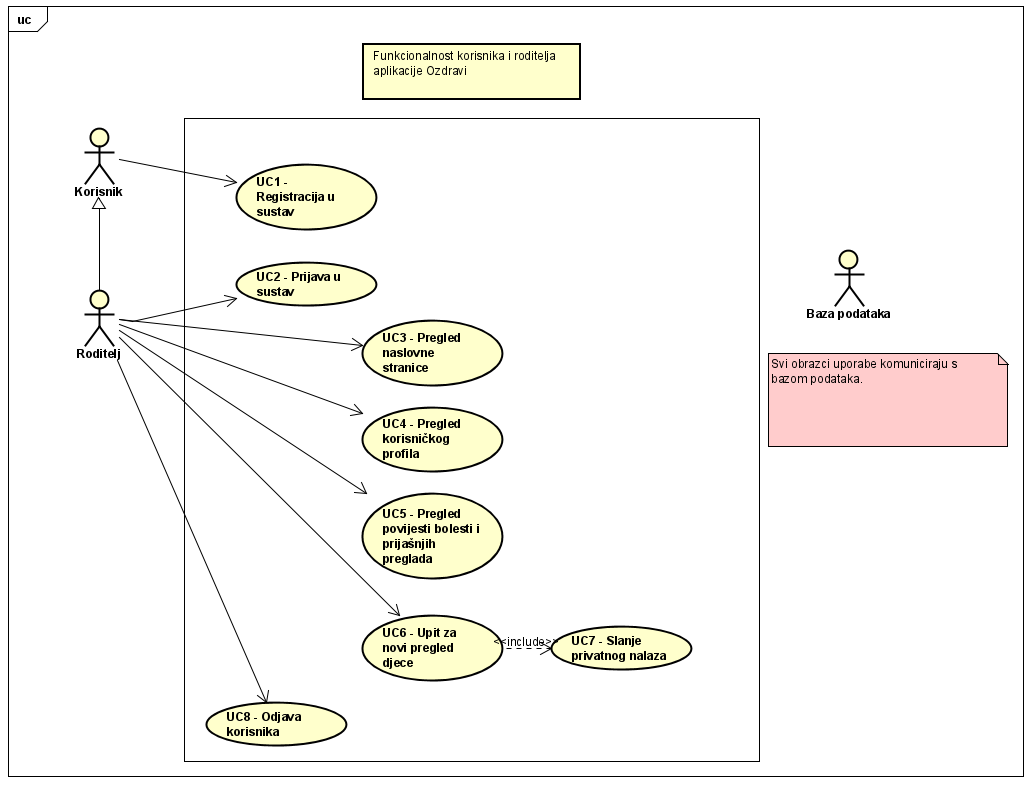
\includegraphics[scale=0.6]{dijagrami/UCRoditelj.PNG}
					\centering
					\caption{Dijagram obrasca uporabe, funkcionalnost korisnika i roditelja}
					\label{fig:myChart}
				\end{figure}
				
				\begin{figure}[H]
					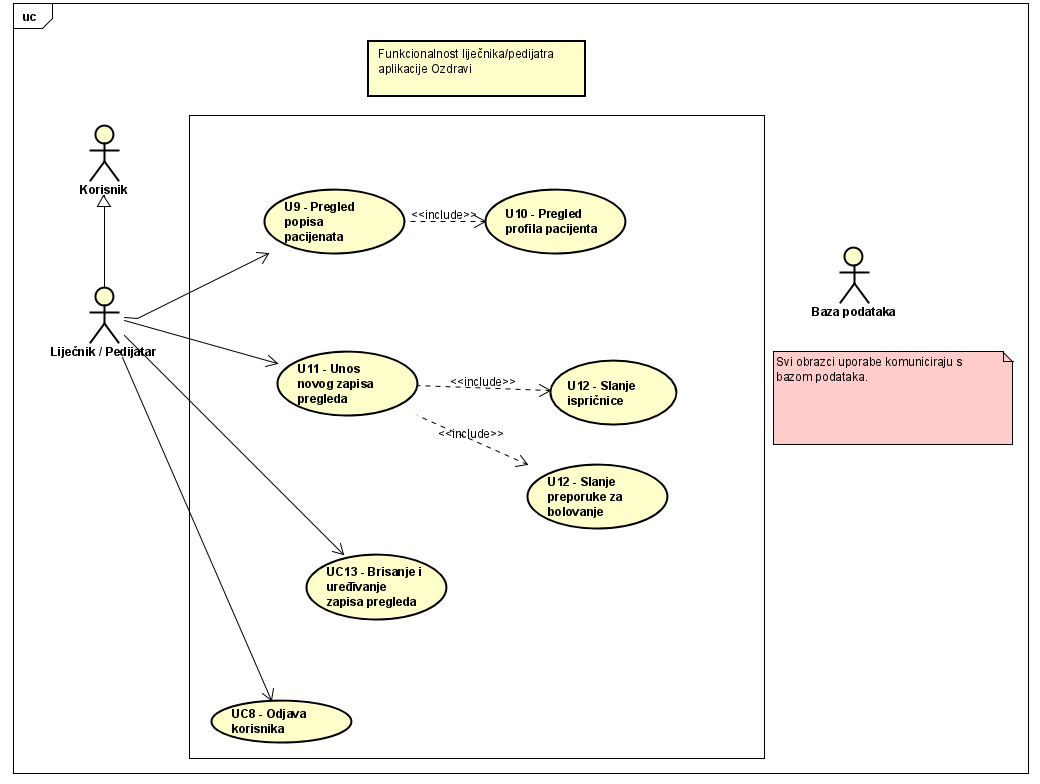
\includegraphics[scale=0.6]{dijagrami/UCLijecnikPedijatar.PNG}
					\centering
					\caption{Dijagram obrasca uporabe, funkcionalnost liječnika/pedijatra}
					\label{fig:myChart}
				\end{figure}
				
				\begin{figure}[H]
					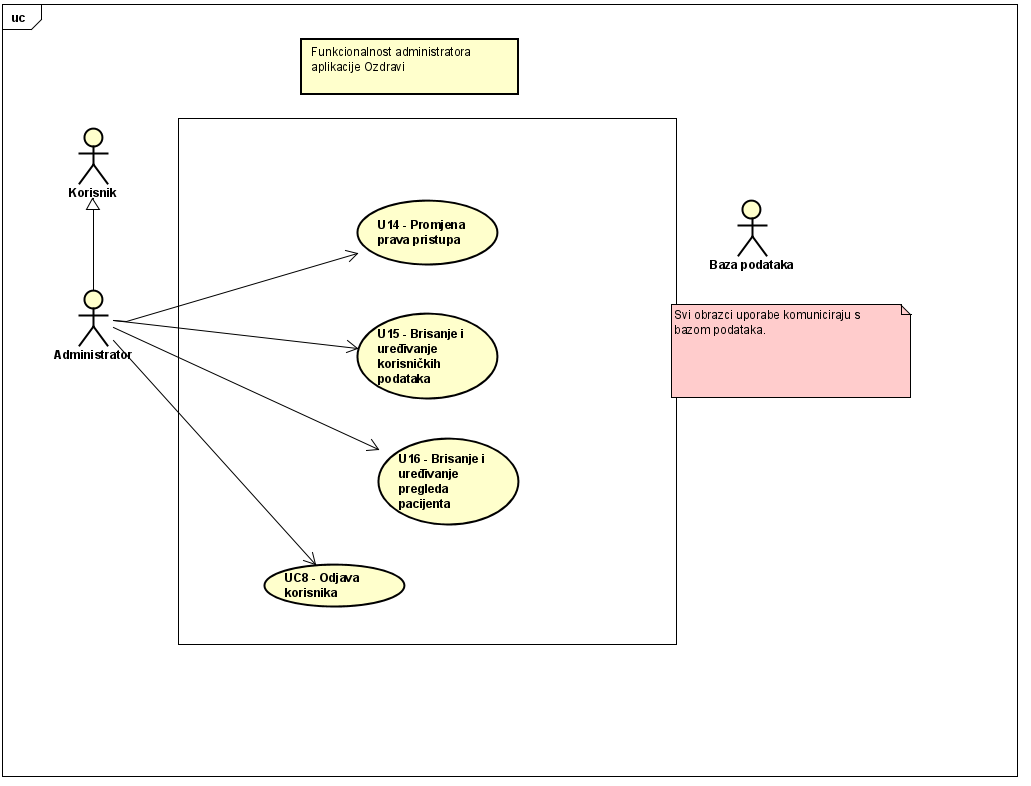
\includegraphics[scale=0.6]{dijagrami/UCAdministrator.PNG}
					\centering
					\caption{Dijagram obrasca uporabe, funkcionalnost administratora}
					\label{fig:myChart}
				\end{figure}
				
			\subsection{Sekvencijski dijagrami}
				
				\subsubsection{Obrazac uporabe U2 - Registracija korisnika}
				Klijent dolazi na stranicu registracije i unosi potrebne podatke za kreiranje računa (ime, prezime, OIB, datum rođenja, adresa, spol, email, lozinka). Ako uneseni podaci ne zadovoljavaju određeni format, javlja se greška o neispravnom formatu, a gumb registracije ostaje neaktivan. Nakon što korisnik unese sve podatke ispravno, omogućava se gumb registracije i šalje se zahtjev za spremanje u bazu podataka. Ako već postoji korisnik s istim emailom ili OIB-om, registracija je neuspješna i opet se javlja greška korisniku. Tek nakon što se unesu OIB i email koji nisu već registrirani, registracija postaje uspješna i korisnik se preusmjerava na naslovnu stranicu.
				
				\begin{figure}[H]
					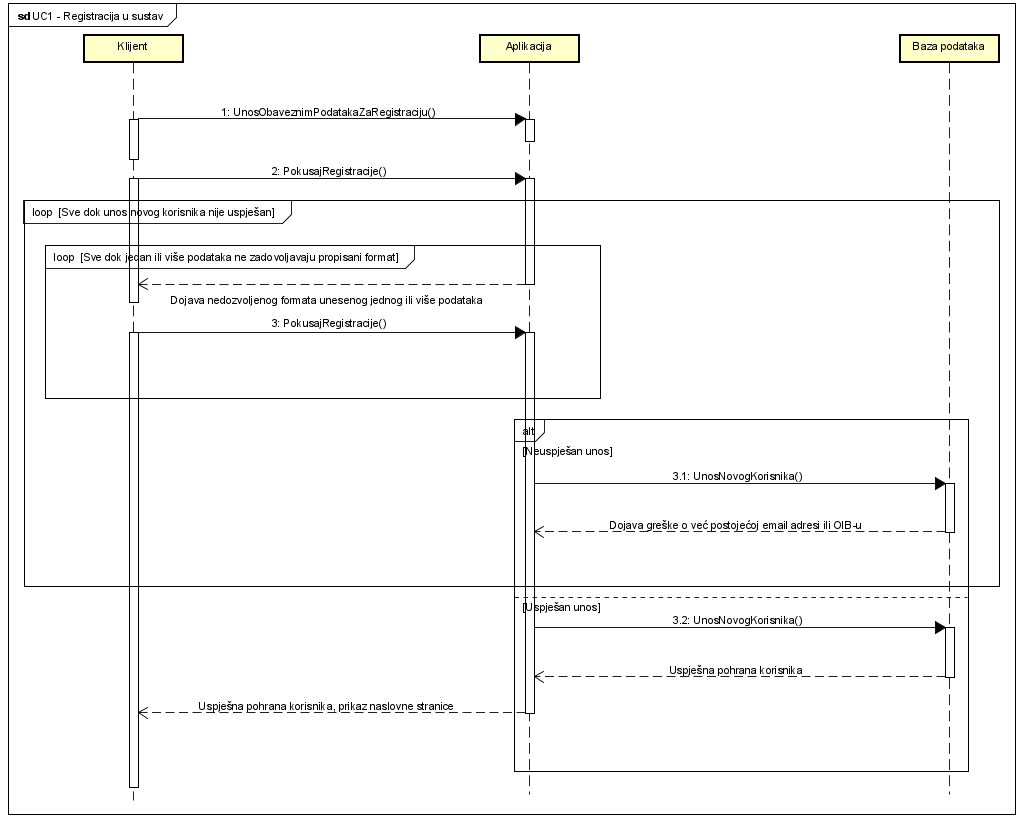
\includegraphics[scale=0.6]{dijagrami/SDRegistracija.PNG}
					\centering
					\caption{Sekvencijski dijagram za UC2}
					\label{fig:myChart}
				\end{figure}
	
		\section{Ostali zahtjevi}
			\begin{packed_item}
			\item	Sustav treba omoguciti rad više korisnika u stvarnom vremenu
			\item	Korisničko sučelje i sustav moraju podržavati hrvatsku abecedu
			\item	Izvršavanje dijela programa u kojem se pristupa bazi podataka ne smije trajati duze od nekoliko sekundi
			\item	Neispravno koristenje korisničkog sučelja ne smije narušiti funkcionalnost i rad sustava
			\item	Sustav treba biti jednostavan za koristenje
			\item	Nadogradnja sustava ne smije narusavati postojeće funkcionalnosti sustava
			\item	Veza s bazom podataka mora biti kvalitetno zastičena, brza i otporna na vanjske greške
			\item	Pristup sustavu mora biti omogucen iz javne mreže pomoću HTTPS
			\end{packed_item}
			 
			 
			 
	
